\begin{problem}{지도 설치}{표준 입력(stdin)}{표준 출력(stdout)}{2\,초}{1024\,MB}

듀벤은 강아지 산책로 사용견들의 편의를 위해서 산책로에 지도들을 설치하려고 한다. 산책로는 여러 개의 정점과 단방향 간선으로 이루어진 그래프로 생각할 수 있고, 서로 다른 출발점과 도착점이 각각 한 개씩 정해져 있다.

정점은 총 $N$개 있으며, 간선은 총 $M$개 있다. $N$개의 정점은 각각 $1$부터 $N$까지의 번호가 부여되어 있다. 출발점은 $S$번 정점이고, 도착점은 $E$번 정점이다. 당신은 $S$에서 출발해 $E$에 도착하는 모든 경로들이 적어도 $K$개의 지도를 거쳐가도록 지로를 설치해야 한다. $S$에서 $E$로 가는 경로가 하나도 존재하지 않는 경우에는, 지도를 하나도 설치하지 않아도 조건을 만족한 것으로 본다.

한 정점에는 지도를 한 개만 설치할 수 있으며, 각 정점마다 지도를 설치하는 데 드는 비용이 다르다. 정점 $v$에 지도를 설치하는 데 필요한 비용은 양의 정수 $C_v$로 주어진다. 출발점과 도착점에도 지도를 설치할 수 있다.

당신은 가능한 최소 비용으로 지도 설치를 완료하고 싶다. 조건을 만족하도록 지도를 설치할 수 있는지를 판별하고, 설치가 가능한 경우에는 최소 비용으로 지도를 설치하기 위해 어떤 정점들에 지도를 설치해야 하는지를 출력하라.

\InputFile
첫 번째 줄에 정점 개수 $N$,  간선 개수 $M$, 최소 지도 개수 $K$가 주어진다. ($2 \leq N \leq 200, 1 \leq M \leq 500, 1 \leq K \leq 5$)

그 다음 줄에는 출발점 $S$와 도착점 $E$가 주어진다. ($1 \leq S,E \leq N, S \neq E$)

그 다음 줄에는 $i$번째 정점의 지도 설치 비용 $C_i$를 나타내는 양의 정수 $N$개가 정점 순서대로 공백으로 구분되어 주어진다. ($1 \leq C_i \leq 10\ 000\ 000, 1 \leq i \leq N$)

그 다음 $M$개 줄에는 $j$번째 간선이 연결하는 두 정점 $u_j\ v_j$가 주어진다. $j$번째 간선은 $u_j$번 정점에서 출발해서 $v_j$번째 정점에 도달한다. ($1 \leq u_j, v_j \leq N, 1 \leq j \leq M$)

주어진 그래프에서 한 정점에서 출발해 동일한 정점에 도착하는 간선이 없음이 보장되며, 임의의 서로 다른 두 정점 쌍 $(u, v)$에 대해, $u \rightarrow v$와 $v \rightarrow u$인 간선은 동시에 입력으로 주어질 수 있지만 $u \rightarrow v$는 최대 한 개, $v \rightarrow u$도 최대 한 개만 입력으로 주어질 수 있다.

주어진 그래프에서 $S$에서 출발해 $E$에 도착하는 경로가 존재하지 않을 수 있음에 유의하라.

\OutputFile
조건을 만족하는 지도 설치가 불가능한 경우, 첫 번째 줄에 $-1$을 출력한다.

조건을 만족하도록 지도 설치가 가능한 경우, 첫 번째 줄에 설치해야 하는 정점의 개수 $P$를 출력한다. ($0 \leq P \leq N$) \newline
두 번째 줄에는 조건을 만족시키기 위해 지도를 설치해야 하는 정점 $P$개를 공백으로 구분하여 출력한다.

\Examples

\begin{example}
\exmp{
3 2 5
1 3
1 60 35
1 2
2 3
}{%
-1
}%
\exmp{
7 11 1
1 7
100 5 7 16 11 12 100
1 2
1 3
1 4
1 5
2 3
2 6
3 6
4 3
4 7
5 7
6 7
}{%
3
5 4 6
}%
\end{example}

\begin{figure}[h]
    \begin{center}
        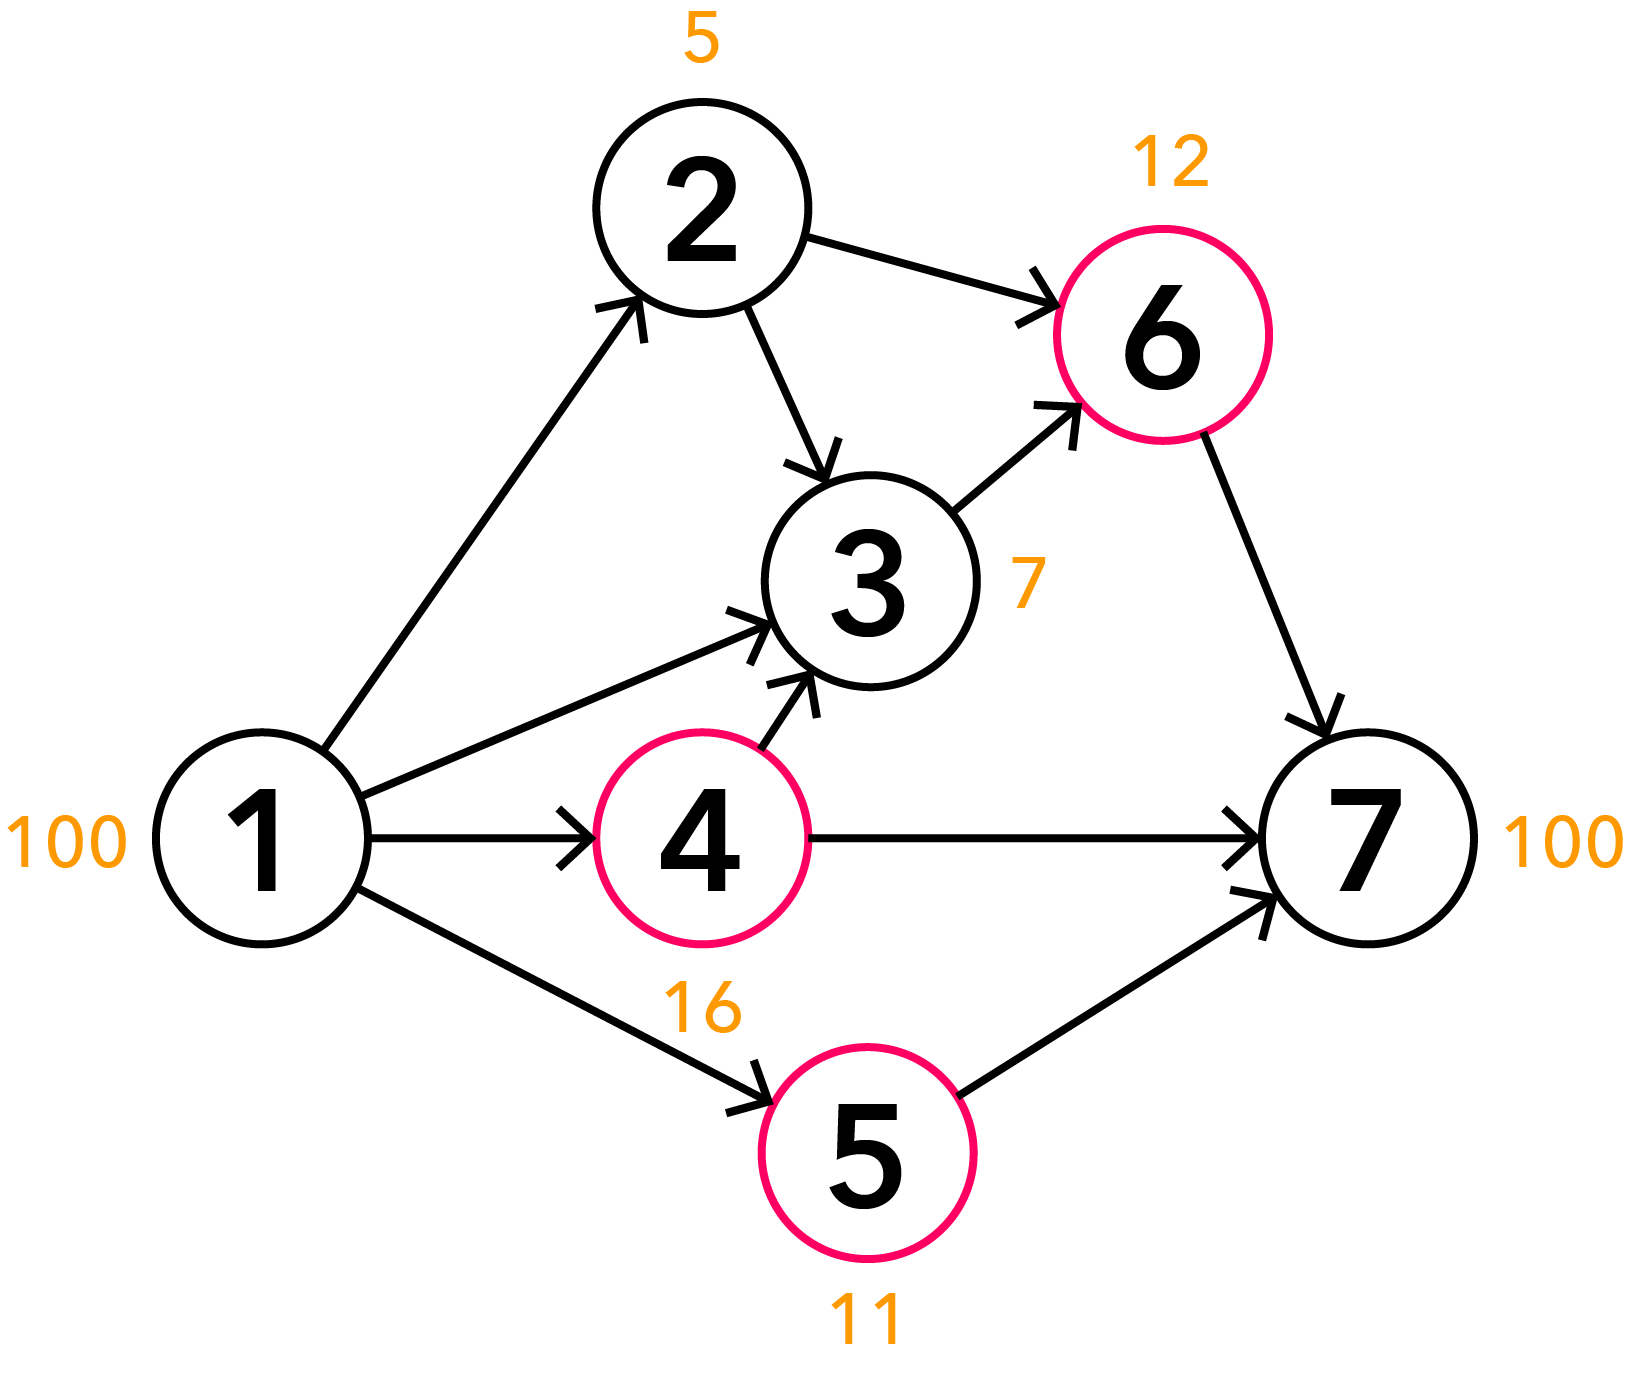
\includegraphics[width=.5\textwidth]{../picture/maps_ex_1.png}
    \end{center}
\end{figure}

\end{problem}
